%% Basierend auf einer TeXnicCenter-Vorlage von Mark Müller
%%%%%%%%%%%%%%%%%%%%%%%%%%%%%%%%%%%%%%%%%%%%%%%%%%%%%%%%%%%%%%%%%%%%%%%

% Wählen Sie die Optionen aus, indem Sie % vor der Option entfernen  
% Dokumentation des KOMA-Script-Packets: scrguide

%%%%%%%%%%%%%%%%%%%%%%%%%%%%%%%%%%%%%%%%%%%%%%%%%%%%%%%%%%%%%%%%%%%%%%%
%% Optionen zum Layout des Artikels                                  %%
%%%%%%%%%%%%%%%%%%%%%%%%%%%%%%%%%%%%%%%%%%%%%%%%%%%%%%%%%%%%%%%%%%%%%%%
\documentclass[%
%a5paper,							% alle weiteren Papierformat einstellbar
%landscape,						% Querformat
10pt,								% Schriftgröße (12pt, 11pt (Standard))
%BCOR1cm,							% Bindekorrektur, bspw. 1 cm
%DIVcalc,							% führt die Satzspiegelberechnung neu aus
%											  s. scrguide 2.4
%twoside,							% Doppelseiten
%twocolumn,						% zweispaltiger Satz
%halfparskip*,				% Absatzformatierung s. scrguide 3.1
%headsepline,					% Trennline zum Seitenkopf	
%footsepline,					% Trennline zum Seitenfuß
titlepage,						% Titelei auf eigener Seite
%normalheadings,			% Überschriften etwas kleiner (smallheadings)
%idxtotoc,						% Index im Inhaltsverzeichnis
%liststotoc,					% Abb.- und Tab.verzeichnis im Inhalt
%bibtotoc,						% Literaturverzeichnis im Inhalt
%abstracton,					% Überschrift über der Zusammenfassung an	
%leqno,   						% Nummerierung von Gleichungen links
%fleqn,								% Ausgabe von Gleichungen linksbündig
%draft								% überlangen Zeilen in Ausgabe gekennzeichnet
]
{scrartcl}

%% Deutsche Anpassungen %%%%%%%%%%%%%%%%%%%%%%%%%%%%%%%%%%%%%
\usepackage[english]{babel}
\usepackage[T1]{fontenc}
\usepackage[utf8]{inputenc}

\usepackage{lmodern} 
\usepackage{paralist} 
\usepackage{microtype} 
\usepackage{graphicx} 
\usepackage{hyperref}


\begin{document}

\pagestyle{empty} %%Keine Kopf-/Fusszeilen auf den ersten Seiten.


\title{Post-Conference Report: ISMIR 2021}
\author{~}
%\and{Der Name des Co-Autoren}
%\thanks{Fußnote}			% entspr. \footnote im Fließtext
%\date{}							% falls anderes, als das aktuelle gewünscht
%\publishers{Herausgeber}
\maketitle 	
\tableofcontents		

\section{Introduction and Personnel}
    The 2021 meeting of The International Society for Music Information Retrieval was the second fully virtual conference that occurred since the beginning of ISMIR, following the virtual conference organized by the team in Montreal in 2020. ISMIR 2021 was conceptualized and planned as an online-only conference due to the COVID19 pandemic. Going completely virtual also offered opportunities to recruit a diverse team from different countries. 

    This report describes the design, organization, execution and results of ISMIR 2021 conference with recommendations for future ISMIR organizers.  

    The sections are organized to present information from each group of chairs. The organization team consisted of the following chairs and people:

    \begin{itemize}
        \item   General chairs: Jin Ha Lee, Alexander Lerch
        \item   Scientific program chairs: Zhiyao Duan, Juhan Nam, Preeti Rao, Peter van Kranenburg
        \item   Diversity and inclusion chairs: Blair Kaneshiro, Jordan Smith
        \item   Technology chairs: Sharath Adavanne, Stefan Balke, Hendrik Schreiber, Fabian-Robert Stöter
        \item   Social program chair: Oriol Nieto
        \item   Tutorial program chairs: Yi-Hsuan Yang, Ashis Pati
        \item   Late breaking demo program chairs: Li Su, Chih-Wei Wu, Siddharth Gururani
        \item   Music program chairs: Carlos Guedes, Bochen Li
        \item   Publications chair: Ajay Srinivasamurthy
        \item   Sponsorship chairs: Sertan \c{S}entürk, Alia Morsi, Lamtharn “Hanoi” Hantrakul
        \item   Social media chair: Qhansa Bayu
        \item   Volunteering chair: Kahyun Choi
        \item   Lab showcases chair: Lele Liu
        \item   Newcomer initiatives chairs: Nick Gang, Elona Shatri
        \item   Website chairs: Ashvala Vinay
    \end{itemize}

\section{Goals and Initiatives Summary}
    Our goal was to ensure that we continue to keep the ISMIR community strong and connected through this unprecedented global challenge. In addition, this year’s ISMIR focused on maximizing the benefit of the online mode in terms of broadening our research and increasing the accessibility to the conference. The following new initiatives were introduced to support those goals: 
    \begin{itemize}
        \item   Increased accessibility to the conference: We wanted to ensure that the registration fee stays low, especially for student participants. Furthermore, we focused on securing funding from sponsors to enable us to offer various kinds of financial support to participants, especially students, women, and caregivers. 
        \item   Newcomer initiatives: There were a number of initiatives such as the newcomer squads, sessions targeted for newcomers, blog posts explaining different aspects of participating in the conference, and LBD session specifically for ``New to ISMIR'' to help encourage participation from people who have never been to ISMIR in the past. 
        \item   Special paper track: A Special Call for Papers focusing on the theme of Cultural Diversity in MIR promoted diversity of MIR research as well as the ISMIR community. 
    \end{itemize}

    Furthermore, the following new initiatives were implemented to enrich our conference experience:
    \begin{itemize}
        \item   Best paper candidate presentation sessions: All the candidates of the best paper awards were given a separate session in which they could give an oral presentation of their work and answer questions.
        \item   Extended social program: Based on survey results from ISMIR 2020 requesting more opportunities to connect with each other, we implemented different social programs such as the use of Gather.town, virtual jam sessions, trivia, etc.
        \item   Lab showcases: To further support the connections between different labs and interested students, we implemented a lab showcase program.
        \item   Instead of using a single conference platform, we used a number of different platforms including Midspace, Gather.town, and Zoom to maximize the benefits of each platform. We focused on putting extra attention to ensure that we minimize the confusion that could arise due to platform switching. 
    \end{itemize}
    
\section{Conference Schedule and Platforms}
    TODO: Not yet available.
    
\section{Diversity, Inclusion, and Newcomer Initiatives}
    \begin{itemize}
        \item \textbf{Personnel}
            \begin{itemize}
                \item   DEI chairs: Blair Kaneshiro, Jordan B. L. Smith
                \item   Newcomer initiative charis: Nick Gang, Elona Shatri
            \end{itemize}
        \item   Timeline
            \begin{itemize}
                \item   Nov 2020: Blair joined 
                \item   Apr 2021: Jordan joined as co-chair
                \item   Aug 2021: Nick and Elona join as Newcomer Initiatives chairs
            \end{itemize}
    \end{itemize}
    
    The workload for the combined D\&I initiatives was very high. If wishing to promote a similar scope of D\&I programming in the following years, chairs are encouraged to consider forming a larger team. For instance, two D\&I chairs who coordinate and advise across initiatives and communicate with GCs, plus subcommittees formed for separate initiatives, e.g., Newcomer Initiatives, Grants, Plenary and Meetup Sessions, Community Engagement (surveys and blog posts).

    \subsection{Aims}
        Our \textbf{high-level} aims were:
        \begin{itemize}
            \item   ensuring a positive and supportive conference environment for all,
            \item   supporting a diverse range of presenters and attendees across backgrounds, locations, career stages, and MIR research areas, and
            \item   taking a broader view of who is supported under the umbrella of D\&I.
        \end{itemize}

        We continued the following initiatives from previous years:
        \begin{itemize}
            \item   We published a Conference Code of Conduct and asked all participants to agree to it.
            \item   WiMIR was represented in the main conference program with keynote and meet-up sessions. (see Sects.~\ref{} and \ref{})
            \item   The WiMIR Workshop (October 29-30) took place as a satellite event. This was not officially planned under the umbrella of “D\&I at ISMIR 2021”, but the D\&I co-chairs (Blair and Jordan) were 2 of the 5 workshop organizers.
            \item   We provided grants to certain categories of attendee, to encourage people from under-represented groups or without means to attend ISMIR. The categories are listed below; those given in italics were introduced this year.
                \begin{itemize}
                    \item   WiMIR,
                    \item   Black in MIR,
                    \item   \textit{Low-income countries},
                    \item   \textit{``New to ISMIR'' Late-Breaking/Demo presenters},
                    \item   \textit{Queer in MIR},
                    \item   Student,
                    \item   \textit{Unaffiliated}
                \end{itemize}
            \item   We solicited WiMIR-specific sponsorship, which this year supported general D\&I efforts (conference fee waivers and child care grants).
        \end{itemize}

        We also planned new initiatives:
        \begin{itemize}
            \item   Authored a series of blog posts to demystify MIR (see Sect.~\ref{}):
               Conducted community surveys and wrote blog posts aiming to demystify paper writing, reviewing, and the conference.
            \item   Held two D\&I meetup sessions (see Sect.~\ref{}):
               Opportunities to engage in discussion with invited ISMIR and WiMIR panelists on current topics of interest. 
            \item   Newcomer Initiatives: blog post and Newcomer Squads (see Sect.~\ref{}):
               These two initiatives were designed to welcome people new to ISMIR to the conference and to the community.
        \end{itemize}


        There were two initiatives that related to D\&I, but which the D\&I co-chairs did not coordinate:
        \begin{itemize}
            \item   New Late-Breaking / Demo track: ``New to ISMIR''
                \begin{itemize}
                    \item   Contributions by junior researchers or practitioners.
                    \item   Submissions mentored by community volunteers providing constructive feedback.
                    \item   20 of 58 LBD submissions this year are ``New-to-ISMIR.''
                \end{itemize}
            \item   Special Call for Papers on ``Cultural Diversity in MIR'' (see Sect.~\ref{})
        \end{itemize}

    \subsection{D\&I and WiMIR Events During ISMIR 2021}
        \subsubsection{WiMIR Plenary Session}
            Decisions and actions:
            \begin{itemize}
                \item   The plenary session consisted of a short presentation about WiMIR and its activities over the past year, followed by an invited keynote talk by Laurel Smith Pardue.
                \item   We invited Dr.\ Pardue due to aligned initiatives between WiMIR/ISMIR and NIME D\&I efforts in 2021, and to bring a neighboring community’s (NIME) perspectives to the ISMIR community. Thus we felt the talk would be relevant both for those interested in D\&I and to the MIR community and for those who are interested in research in neighboring communities.
                \item   Payment: Dr.\ Pardue was paid the same honorarium as the two main keynote speakers.
            \end{itemize}

            Timeline:
            \begin{itemize}
                \item   Apr 2021: List of keynote speaker candidates
                \item   Jul 2021: Keynote speaker identified, invited, and confirmed.
                \item   Oct 2021: Finalization of schedule
                \item   Jan 2022: Honorarium payment 
            \end{itemize}

            Recommendations:
            \begin{itemize}
                \item   Make sure that the WiMIR plenary session remains a part of the main conference program (as it has been since ISMIR2015). 
                \item   It is at the discretion of the WiMIR/D\&I chairs to decide the format of the session. Past sessions have included presentations on WiMIR initiatives (ISMIR2016), other community presentations (ISMIR2018), and invited keynotes (ISMIR2017, ISMIR2019, ISMIR2020, ISMIR2021). 
                \item   If inviting an external keynote speaker, coordinate with the general chairs to discuss financial support (e.g., honoraria, travel funds) and which funding bucket it comes out of.
                \item   Plan the honorarium payment in advance of the conference so that funds can be paid without delay after the conference.
            \end{itemize}

    \subsection{D\&I Meetup Sessions}
        Special WiMIR-themed meet-up sessions were introduced in the virtual ISMIR 2020 conference. In these ``Notable Women in MIR'' sessions, conference attendees could engage in informal discussion and Q\&A with an invited woman in the field. The ISMIR 2021 conference continued this tradition. The ISMIR 2021 conference additionally included, for the first time, two meet-up sessions structured as panel discussions that were focused on broader topics relating to D\&I in MIR.
        
            Decisions and actions:
            \begin{itemize}
                \item   We were allocated 2 meetup sessions per day of the main conference (8 slots total).
                \item   We transferred the 2 slots on Day 1 to the Newcomer Initiatives team, who hosted sessions on ``Getting the most out the ISMIR conference'' (see Sect.~\ref{}).
                \item   We allocated the 4 slots on Day 2 and Day 3 for ``Notable women in MIR'' sessions with an invited presenter in each one. (Info: \href{https://ismir2021.ismir.net/wimir}{https://ismir2021.ismir.net/wimir}).
                \item   We allocated the 2 slots on Day 4 for broader topics: One on ``Broadening D\&I'' and one on ``Local initiatives.'' These were each a panel format, with one of the D\&I chairs moderating a panel of four invited panelists.
                \item   We sought a slate of guests and panelists to represent a variety of research areas, academic/industry affiliations, career stages, and geographic locations.
            \end{itemize}

            Timeline:
            \begin{itemize}
                \item   Summer 2021: Discussion on how to program the 8 meetup sessions. One alternative was to allocate 2 sessions each to ``Newcomers,'' ``Women in MIR,'' ``Black in MIR,'' and ``Queer in MIR.''
                \item   Sep 2021: Final session topic allocation.
                \item   Oct 2021: Identification and invitation of ``notable women'' and panel members.
            \end{itemize}

            Recommendations:
            \begin{itemize}
                \item   The ISMIR2022 chairs are encouraged to seek meet-up slots throughout the conference to program as they wish.
                \item   For the ``Notable Women in MIR'' sessions, we invited the four presenters seeking variety in geographical location and academia/industry representation. We were also mindful not to re-invite anyone who had already presented in these sessions in 2020.
            \end{itemize}

            Programming details:
            \begin{itemize}
                \item   Special WiMIR-themed meet-up sessions were introduced in the virtual ISMIR 2020 conference. In these ``Notable Women in MIR'' sessions, conference attendees could engage in informal discussion and Q\&A with an invited woman in the field. The ISMIR 2021 conference continued this tradition, allocating four D\&I meet-up sessions for ``Notable Women in MIR'' sessions with invited presenters Cheng-Zhi Anna Huang (Magenta / Google Brain / Université de Montréal / Mila), Emma Azelborn (iZotope, Inc.), Xiao Hu (The University of Hong Kong), and Katerina Kosta (ByteDance / TikTok).
                \item   The first session, focused on ``Broadening D\&I,'' included invited panelists Johanna Devaney (Brooklyn College and the Graduate Center, CUNY; WiMIR organizer; former ISMIR conference organizer), Zhiyao Duan (University of Rochester; ISMIR conference organizer), Katie Kinnaird (Smith College; former WiMIR organizer; former ISMIR conference organizer), and Doug Turnbull (Ithaca College; former ISMIR Board member; former ISMIR conference organizer). 
                \item   The second session, focused on ``Local Initiatives,'' included invited panelists Sakinat Folorunso (Olabisi Onabanjo University; IndabaX Nigeria organizer), Meinard Muller (International Audio Laboratories Erlangen; ISMIR Board President), Elio Quinton (Universal Music Group; London Audio \& Music AI Meetup organizer; WiMIR mentor), and Anja Volk (Utrecht University; former WiMIR organizer; TISMIR co-founder). Each panel was moderated by one of the D\&I chairs.

            \end{itemize}
    \subsection{D\&I Organizing Responsibilities}
        In addition to organizing the above events during the conference, we also were responsible for other items.
        
        \subsubsection{Conference Code of Conduct}
            The Code of Conduct was introduced for ISMIR2018 and is a joint effort between the conference organizers and the ISMIR Board.
            
            Decisions and actions:
            \begin{itemize}
                \item   We iterated on the ISMIR2020 Code of Conduct, which had already been updated for the virtual format.
                \item   There was one Code of Conduct complaint filed and investigated during the conference.
            \end{itemize}

            Timeline:
            \begin{itemize}
                \item   Apr 2021: Code of conduct edited by D\&I chairs in April 2021
                \item   Apr 2021: Draft shown to General Chairs and ISMIR Board.
                \item   May 2021: Code of conduct posted to website.
            \end{itemize}

            Recommendations:
            \begin{itemize}
                \item   The Code of Conduct will need to be updated to account for a hybrid conference format (likely incorporating content from ISMIR2018-2019 in-person and ISMIR2020-2021 online versions).
            \end{itemize}

        \subsubsection{Registration and Childcare Grants}
            TODO: [see blog post for background]
            
            TODO: [see WiMIR plenary intro slides for outcomes]

            TODO: Recommendations for future ISMIR conferences
            
        \subsubsection{D\&I Blog Posts}
            TODO: [see blog post for motivation]

            TODO: [see blog page for posts]

            TODO: Thank survey respondents

            TODO: Recommendations for future ISMIR conferences
            
        \subsubsection{D\&I Collaborations with Other Organizers}
            The Diversity \& Inclusion efforts of the ISMIR 2021 conference were not limited to the D\&I chairs. The following chairs were most notably involved
                \begin{itemize}
                    \item   General Chairs: Scoping initiatives, seek feedback on new initiatives
                    \item   Program Chairs / Special call for papers: Gave feedback throughout process
                    \item   LBD Chairs / Special LBD track: Gave feedback on call, coordinated to handle grants
                    \item   Sponsorship Chairs / WiMIR Sponsorship: We are grateful to the Sponsorship chairs for taking the lead on WiMIR Sponsorship
                    \item   Web and PR Chairs: Constant communication to keep web and social media updated with D\&I / Newcomer initiatives, and thanking WiMIR sponsors
                \end{itemize}

            TODO: Recommendations for future ISMIR conferences
            
    \subsection{Newcomer Initiatives}
        TODO: General intro to why we do this

        TODO: ``Getting the Most Out of ISMIR'' Blog Post
        \begin{itemize}
            \item   TODO: Why we did this, what we did, what it produced
            \item   TODO: Thank survey respondents
            \item   TODO: Recommendations for future ISMIR conferences
        \end{itemize}

       
        TODO: Newcomer Squads
        \begin{itemize}
            \item   TODO: Why we did this, what we did, what it produced
            \item   TODO: Thank the squad leaders who volunteered their time for this new initiative
            \item   TODO: Recommendations for future ISMIR conferences
        \end{itemize}
        

    \subsection{Collaborations with Other WiMIR Initiatives}
        Finally, the broader initiatives of the WiMIR community tied in to the ISMIR 2021 D\&I initiatives. The 5th Annual WiMIR Workshop, which took place virtually in October 2021, was again an official satellite event of the ISMIR conference. The ISMIR 2021 D\&I chairs coordinated with WiMIR Mentoring Program organizers to obtain statistics on the program for the WiMIR plenary session, and to announce the opening of the 2022 round sign-ups during the conference. Finally, the ISMIR 2021 team cross-posted existing content from the WiMIR Blog to further highlight content by and about women in the field. 

        Future ISMIR organizers can continue to maintain open channels of communication with organizers of the WiMIR Workshop, WiMIR Mentoring Program, and WiMIR Blog in order to promote visibility of these initiatives to ISMIR conference attendees.

    
\section{Conference Program}
    \subsection{Papers}
        This section lists some learnings/observations/comments based on the experiences of the 2021 PC team. This might help to improve the submission and review process in future ISMIRs. These are rough notes and not ordered in a specific manner.
        
        \subsubsection{Submission Process}
            \begin{itemize}
                \item Convey the differences between abstract deadline and final deadline clearly, in terms of what things (author names, order, title, abstract, e.g.) can be changed from abstract deadline to final deadline.
                \item   Establish criteria for desk rejects clearly and ahead of submission (anonymity violations, formatting violations, length violations).
                \item   Instruct authors to clearly add domain and individual CoIs when they submit.
            \end{itemize}
        
        \subsubsection{Review Process}
            \begin{itemize}
                \item   We sought additional reviewers from meta-reviewers, by sharing the existing list of reviewers. To make suggestions better, also add the list of meta-reviewers to that list of reviewers and share it with meta-reviewers. This will ensure meta-reviewers do not suggest reviewers who are already meta-reviewers.
                \item   While adding new people to be invited as meta-reviewers or reviewers, check if they are already on the list of reviewers or meta-reviewers, respectively to avoid double invitations.
                \item   Add a buffer for reviewer/meta-reviewer invitation expiry dates on CMT (compared to what is suggested on the invitation) so that invitees can accept even after the proposed deadline. This will avoid resending invitations to people who wish to accept after the deadline but can’t since the invitation link has expired.
                \item   Some reviewers suggested adding an non-informative option (e.g., “don’t know”) in the multiple-choice categories of review questions, in addition to “strongly agree”, “agree”, “disagree” and “strongly disagree” options. This is to follow the Mutually Exclusive and Collectively Exhaustive (MECE) criteria (\href{https://science.sciencemag.org/content/185/4157/1124}{https://science.sciencemag.org/content/185/4157/1124}) and to avoid inappropriate anchoring of their decisions. We think this is a good suggestion, but the wording of this non-informative option needs to be carefully thought to prevent reviewers from abusing this option.
                \item   Some reviewers indicated a desire to be able to submit supplementary materials with their reviews; This would be helpful for authors to improve their work. We think this is a good suggestion.
                \item   Some authors and reviewers suggested that the ISMIR community needs to be more inclusive for novel applied research, i.e., work that applies existing techniques (often from other fields) in new applications in MIR. They complained that some reviewers viewed such work as “lego-block work” instead of proposing novel theories or methods and expressed a negative tone in their reviews. They made a good point that such applied research is important in demonstrating impacts of theoretical work in MIR, and that there are many other venues where novel theories and applications can be published, yet ISMIR is among the few places where novel MIR applications can be published.
                \item   Similar to ISMIR 2020, we did not install a rebuttal mechanism in ISMIR 2021. We also removed the author feedback form from ISMIR 2020 that was designed for authors to voice in case they strongly feel unfair treatment; This is because this form did not work well and it was not meant to change the review result. Nonetheless, we received several emails complaining about the reviews and it was not easy to respond to each of the authors and persuade them. We believe that adding a rebuttal mechanism might be helpful for resolving these rare but important issues.We note that ICASSP 2022 installed a rebuttal mechanism for the first time, and it seemed to work well.
            \end{itemize}
        
        \subsubsection{Special Call for Papers}
            We think that the special call for papers on cultural diversity in MIR research was successful. This is reflected from the amount of submissions we have received (40 special call submission among the overall 278 submissions). The main feedback and reflection we have is that the review criteria for the special call might be too strict (or less suitable). We designed the special call so that all submissions went through exactly the same review process and were evaluated using the same criteria. However, some authors and reviewers complained that certain reviews were too strict due to unconscious biases. In-depth discussions about these issues among community members were held in Special Session 3. We recognize such biases, and suggest future organizers of this special call or other special calls to consider these issues. Possible ways to address these issues include 1) raising the awareness of such issues in communications with reviewers, 2) add questions in the review form that are suited to judgment criteria for the special call, and 3) implement “affirmative action” type of mechanisms in the final decision process.

        \subsection{Notes from 2020 chairs}
            We computed the overall scores by adding more weight to the meta-reviewers' scores and sorted them to find the cutoff point. This is because we believe meta reviewers have more experience and expertise whereas some of the reviewers are new/less experienced, so we want to balance it out.
            Then the PC members divided the list of all papers into two batches, and each member reviewed the decisions to ensure that there was no red flag. The kinds of things we looked for, for instance, are meta-reviewers overturning all three reviewers' decision, huge variance in review score (strong reject \& strong accept), cases where the reviewer left poor quality review (one line review), cases where the meta-reviewers specifically asked for help, cases where the reviewers' did not seem to have enough expertise to evaluate the paper well, etc.

            If the decision looked reasonable, we would just mark okay, and if there was something odd about the case, we would mark it "to discuss" and discussed the item as a group.

            We also discussed the borderline papers that could go either way. For this, we tried to make our best judgment given the reviews, discussion, and what we believed is the value of the paper (e.g., valuable data set? new perspectives?).
            
            After informing the decision, we did receive several requests to reconsider the final decision based on unfair review, etc. Overturning the decision does happen, but not frequently and only when there is a reason that made sense to all the PC members.

    \subsection{Special Sessions}
        PCs came up with the topics of special sessions, considering issues that are timely and broadly impacts the MIR community. PCs invited a senior researcher who is experienced and active for each topic as a moderator, and asked him/her to invite panelists and write an abstract. The special sessions were generally well-received with positive responses from the moderators and panelists. 

        A tricky part in organizing the special sessions was scheduling the time because the sessions are allocated to the remaining times slots in the program and the moderator/panelists are in different time zones. PCs had to closely communicate with the moderators to fix the schedule.


        \subsubsection{Special Session 1: MIR for Human Health and Potential Panel}
        \begin{itemize}
            \item Time: 3:30-4:30 AM on November 9, 2021 (UTC)
            \item   Moderator: Ye Wang, National University of Singapore, Singapore
            \item   Panelists: Frank Russo (Ryerson University, Canada), Elaine Chew (CNRS – STMS (IRCAM), France), Gus Xia (NYU Shanghai, China), Blair Kaneshiro (Stanford University, USA)

        \end{itemize}
        
        \paragraph{Closing Remarks}
        \begin{itemize}
            \item   The COVID?19 pandemic has made music more important as a medium to connect people, to enhance both physical and mental health, and to advance human potential
            \item   Social distancing measures have greatly enhanced interest in eHealth and eLearning
            \item   Integrating music into digital health/learning technologies helps to make music interventions accessible, scalable, and personalized
            \item   Research at the intersection of neuroscience, medicine, the science of learning, and MIR has the potential to reveal new insights into individual variability and personalized interventions
            \item   Mobile systems for collecting physiological data point to promising avenues for ecologically valid studies, and even socially distanced data collection in the home
            \item   Our panelists have already shown that it is possible to match their research interests to address important problems in the direction of human health and potential
            \item   Future plans
                \begin{itemize}
                    \item   One hour is certainly too short for an in?depth discussion of such an important topic. We hope to form a SIG within the community to continue the discussion offline, and more regularly.
                    \item   Perhaps we could consider a workshop in ISMIR2022, or a Dagstuhl?style seminar next year.
                    \item   If you are interested in our future discussions, please send me an email to wangye@comp.nus.edu.sg

                \end{itemize}
        \end{itemize}
        
 
        \subsubsection{Special Session 2: IMS Digital Musicology Study Group}
        \begin{itemize}
            \item   Time: 3:30-5:00 PM on November 9, 2021 (UTC)

            \item   Moderators: Johanna Devaney (Brooklyn College and the Graduate Center, CUNY, USA) and Frans Wiering (Utrecht University, The Netherlands)
        \end{itemize}


        \subsubsection{Special Session 3: Promoting Cultural Diversity in MIR Research}
            \begin{itemize}
                \item   Time: 4-5 AM on November 10, 2021 (UTC)

                \item   Moderator: Scientific Program Co-Chairs

                \item   Panelists: Magdalena Fuentes (New York University, USA), Xiao Hu (The University of Hong Kong, Hong Kong), Patrick Savage (Keio University SFC, Japan), Li Su (Academia Sinica, Taiwan)


            \end{itemize}
            
            \paragraph{Summary}
                We had panelists from diverse backgrounds (Li Su from information technology, Patrick Savage from music cognition, anthropology, Xiao Hu from education and information sciences) who all brought valuable perspectives informed by their own unique experiences. They all agreed that the need for cultural diversity in music studies is important beyond argument, and that this year’s special call is a step in the right direction for promoting cultural diversity in the ISMIR scientific program. However, a lot remains to be done for it to achieve its goal. Also while we’re now seeing a small but growing representation of researchers from East Asia, this is not true for Africa and South America, for instance.
                
                \textit{Challenges in cross-cultural research initiatives} are mainly
                    \begin{itemize}
                        \item   the necessity for cross-disciplinary collaborations. This tends to be more arduous than engaging with colleagues from within a discipline and therefore has a high entry barrier. Even more difficult is the proposed ‘technology+arts’ combination typical of our work. Making the rewards for such research contributions more attractive (e.g. by increasing their visibility in conferences/journals) would help to an extent. 
                        \item   Scarcity of datasets. The ISMIR community can play a role in applying their collective expertise to the creation and dissemination of cross-cultural datasets and resources (i.e., purporting to non-Western music or populations). 
                    \end{itemize}
                
                \textit{Improving the acceptance rates of cross-cultural research submissions}: Several suggestions were made that can be broadly categorized as follows.
                    \begin{enumerate}
                        \item   Implementing some form of ‘affirmative action’.  While most were not in favour of the straightforward relaxation of acceptance criteria, everyone agreed that new criteria need to be considered while re-weighting some of the current criteria. The current standards have worked well for the mainstream but continuing to judge with the same standards will not help diversification. Given the challenges in defining problems and approaches in heretofore unexplored areas, it is not reasonable to enforce the (traditionally important) ‘technical novelty’ criterion. Instead, clear evidence of the work helping to define and open up new avenues for research, critical analyses of the inadequacies of current methods and differences in the nature of the dataset and the study with reference to mainstream MIR research must all be considered valuable contributions that serve the cause of diversity well.
                        \item   Finding reviewers: Given the cross-disciplinary expertise typically required to assess such work, we should consider onboarding reviewers who are otherwise typically outside the community. Finally, our acceptance criteria should be explicitly explained to reviewers/meta-reviewers. E.g. a valid criterion for acceptance could be that the work has at least one nice contribution related to cross-culture studies and overall is technically sound.
                        \item   Mentoring: given how supportive the ISMIR community is, we should come up with good mentoring (‘shepherding’) programs to encourage those inclined towards cross-cultural research topics to shape their work into a format that is well suited to ISMIR.  This may be achieved with early deadlines for first submission to be followed up with a revised submission based on mentor comments for the main review.
                    \end{enumerate}


        \subsubsection{Special Session 4: Computational Creativity for Music}
        \begin{itemize}
            \item Time: 2:30-3:30 PM on November 10, 2021 (UTC)

            \item   Moderator: Tom Collins (University of York, UK, Music Artificial Intelligence Algorithms, Inc., USA)

            \item   Panelists: Anna Jordanous (University of Kent, UK), Dan Ventura (Brigham Young University, USA), Geraint Wiggins (VUB, Belgium / Queen Mary University of London, UK), and Portrait XO (Artist)
        \end{itemize}

        \subsubsection{Special Session 5: MIR for Music Education}
        \begin{itemize}
            \item   Time: 4-5 PM on November 10, 2021 (UTC)
            \item   Moderator: Roger Dannenberg (Carnegie Mellon University, USA)
            \item   Panelists: Zhiyao Duan (University of Rochester, USA), Anssi Klapuri (Yousician, Finland), Alexander Lerch (Georgia Institute of Technology, USA), Daniel Ray (Muse Group, UK)

        \end{itemize}

        \subsubsection{Special Session 6: Ethical issues in Music AI --- Perspectives on authorship with creative artificial intelligence in music}
        \begin{itemize}
            \item   Time: 2.30-3.30 PM on November 11, 2021 (UTC)
            \item   Panelists: Andre Holzapfel (KTH Royal Institute of Technology, Sweden), Petra Pauliina Jääskeläinen (KTH Royal Institute of Technology, Sweden), Anna-Kaisa Kaila (KTH Royal Institute of Technology, Sweden), Sertan \c{S}entürk (Kobalt Music Group, United Kingdom) 
        \end{itemize}

    \subsection{Late Breaking Demos}
        \subsubsection{Implemented Changes}
            The main objectives of ISMIR 2021 LBD session were: 1) to fully leverage the online format and increase the number of participants, and 2) to explore the possibility of having a light-weight review process. The idea was to invite more people into our community while maintaining the quality of submissions via peer review. The initial proposal was to implement the peer-review process in LBD, which could potentially face the following challenges:

            \begin{itemize}
                \item   The peer-review process is time-consuming, and it adds additional workload to the ISMIR reviewers.
                \item   It will force an early schedule for LBD, which defeats the purpose of “Late-breaking” demos. 
                \item   People may confuse LBD papers with the official peer-reviewed publications.
                \item   A peer-review process could potentially reduce the number of participants instead of increasing it.
            \end{itemize}
            
            After several discussions, we re-adjusted the goals and introduced the following changes:
            \begin{enumerate}
                \item New-to-ISMIR special track:
                    \begin{itemize}
                        \item We welcome submissions from junior researchers with this opt-in track. All submissions under this track will receive a mentoring process (i.e., a light-weight review process) and financial support (i.e., a registration waiver).

                        \item   The implementation of this special track allows us to assess the possibility and benefit of having a peer-review process in LBD. Ideally, the mentoring process should allow the authors to improve their final manuscripts based on the mentors’ (i.e., reviewers) constructive feedback.  
                        \item   More information can be found in the Call for papers and Mentor's guideline: 
                            \begin{itemize}
                                \item \href{https://ismir2021.ismir.net/clbd/#special-opt-in-track-new-to-ismir}{https://ismir2021.ismir.net/clbd/\#special-opt-in-track-new-to-ismir}
                                \item \href{https://ismir2021.ismir.net/lbd_mentor_guidelines/}{https://ismir2021.ismir.net/lbd\_mentor\_guidelines/}
                            \end{itemize}

                        \item   No upper limit of accepted demos: 
                            \begin{itemize}
                                \item We remove the upper limit (usually capped at 50 in the previous years) for the total number of accepted papers since there is no physical constraint (i.e., the required space for hosting all the posters).

                                \item   We encourage the submission of demo videos during the review process; these videos are also uploaded to midspace as supplementary materials. 
                            \end{itemize}
                    \end{itemize}
            \end{enumerate}

        
            With these changes, we successfully reached our goals with the following stats: 
            \begin{itemize}
                \item   We have a total number of 58 LBD papers, a significant increase from last year. Also, this is the highest number in the past six years (e.g., numbers were 48, 41, 49, 50, 50, 27 from 2015~2020). 20 of which are New-to-ISMIR papers.
                \item   We invited 49 people from the ISMIR reviewer pool to serve as the mentors; 21 people accepted, 22 people did not respond, and 6 people declined. The number of volunteers is sufficient for covering the number of submissions from the New-to-ISMIR track.

                \item   All the authors submitted under the special track received registration waiver. This was made possible due to the support from the Diversity and Inclusion team and the industrial sponsorship from Netflix. 
            \end{itemize}
        \subsubsection{Post-Conference Survey}
            To evaluate the effectiveness of our new initiatives, we sent out a post-conference survey to all the mentors and mentees who participated in the New-to-ISMIR special track. Some highlights from the survey are:
            \begin{itemize}
                \item Mentors:
                    \begin{itemize}
                        \item   We received 5 responses from the mentors
                        \item   In general 2 assignments is good
                        \item   Should recommend mentors to spend less than 2 hours per submission
                        \item   2 weeks review timeline works for all
                        \item   Most mentors liked the introduction of New-to-ISMIR
                        \item   One mentor would have liked a more interactive mentoring process
                        \item   Another had concerns about the quality, and the fact that they felt like they were doing an advisor's job
                    \end{itemize}
                \item   Mentees:
                    \begin{itemize}
                        \item   We received 7 responses from the mentees
                        \item   2 reviews per submission were welcome. Some would have liked 3 reviews
                        \item   Mixture of short term and long term feedback was received
                        \item   Majority would have preferred feedback on long term improvement
                        \item   Mixed results for 1 week camera ready timeline. 1 week was the majority vote but it depended on the feedback
                        \item   All mentees liked the New-to-ISMIR idea
                        \item   All mentees preferred the mentoring process compared to the financial aid
                    \end{itemize}
            \end{itemize}

            In summary, the feedback we received from both mentors and mentees were mostly positive. Based on the responses, we think this special track is effective in introducing new people to our community. Additionally, it also shows that a light-weight peer review process is generally fitting for this purpose. 
        
        \subsubsection{Recommendations for future LBD chairs}
            Timeline:
            \begin{itemize}
                \item   06/13/2021: 1st call for LBD (5 months before conference)
                \item   07/19/2021: 2nd call for LBD (3 months before conference)
                \item   08/30/2021: 3rd call for LBD and submission system open (2 months before conference)
                \item   10/04/2021: Final call for LBD (one week before the submission deadline)
                \item   10/11/2021: Submission deadline (The 4-week timeframe is recommended for future LBDs if a similar review process is implemented. Otherwise, one week before the conference should be sufficient.)
                \item   11/01/2021: Camera-ready submission deadline (We encountered a few late submissions. If future LBDs opt for a similar mentoring process, then the deadline is suggested to be earlier by 48--72 hours.)
            \end{itemize}
            
            During the Event:
            \begin{itemize}
                \item Glitches with Zoom links: to enable audio sharing, we provided presenters the option to use zoom links instead of the default midspace chat room. This last minute notification seemed to create some confusions as well as technical troubles during the conference. For future (online) LBDs, we suggest to provide this alternative solution only upon requests (as opposed to giving this option widely). 
            \end{itemize}
            
            Other feedback:
            \begin{itemize}
                \item   LBD latex template: since LBD papers are not official publications, a potential cosmetic change could help people differentiate LBD papers (i.e., extended abstracts) from the actual ISMIR papers. 
                \item   Poster format: some authors suggested that landscape is better than portrait for an online conference.
            \end{itemize}
    
    \subsection{Tutorials}
        \subsubsection{Soliciting and evaluating tutorial proposals}
            \begin{itemize}
                \item Call for tutorial proposal website: \href{https://ismir2021.ismir.net/cft/}{https://ismir2021.ismir.net/cft/}
                \item   Timeline:
                    \begin{itemize}
                        \item   04/09/2021: Initial Proposal Submission
                        \item   04/16/2021: Final Proposal Submission
                        \item   06/04/2021: Notification of Acceptance
                    \end{itemize}
                \item   We (the tutorial chairs) aimed to accept around 6 tutorials, and we thought it might be good if 3 or 4 of them are invited ones
                \item   We brainstormed and created a list with potential invited speakers, and decided who to invite first.  We took into account factors such as the novelty of the tutorial topic in view of the recent editions of ISMIR, the expertise of the speaker, coverage of different tutorial topics etc.
                \item   In our invitation letter, we encouraged the invited individual to form a team 
                \item   We invited five and four responded and submitted a proposal
                \item   In the meanwhile, we got tutorial proposals from another six teams (that we did not invite)
                \item   The tutorial chairs evaluated the proposals separately, rating them according to the evaluation criteria listed in the call for tutorial proposal website and listing the strengths and weaknesses, and discussed them one-by-one in an online meeting, especially the edge cases.
                \item   Finally we decided to accept all the four invited proposals, plus two non-invited ones.
                \item   We encouraged one of the rejected proposals to consider organizing a special session instead, mainly because the topic of that tutorial proposal can be of interest to a relatively smaller group of ISMIR participants, and partly because it partially overlaps with an invited (and accepted) tutorial content-wise.
                \item   We made sure that we keep in touch with the tutorial speakers before and during the ISMIR conference, asking their needs of technical support, arranging time slots for them to test the video-conferencing platforms, etc.

            \end{itemize}

        \subsubsection{Tutorial Scheduling}
            \begin{itemize}
                \item   Due to the online format of the conference, each tutorial is supposed to have two sessions, which we called session A and session B, so that participants from different time zones may have the chance to take part in at least one of them.

                \item   We created a google sheet and figured out six possible time slots for the proposal (\href{https://docs.google.com/spreadsheets/d/1qPUy-69GDe-Hoo7AvFkFofvxCdZQssBgtf5RAILmPHs/edit#gid=0}{https://docs.google.com/spreadsheets/d/1qPUy-69GDe-Hoo7AvFkFofvxCdZQssBgtf5RAILmPHs/edit\#gid=0}) 

                \item We internally discussed which time slots would be the best for different teams of tutorial speakers, considering their time zones.  (For example, to avoid asking a speaker to present in his/her midnight)

                \item   But, we decided later on to let the tutorials speakers tell us their preferences: we let them know the six slots and asked their preferences.  We then finalized the schedule considering all the speakers’ preferences.

                \item his is the message we sent to them: ``In order to accommodate participants from different time-zones, we will have the tutorials conducted in two sessions: Session A  and Session B. Similar to last year, each tutorial will be presented once in each session. In order to schedule this efficiently, we request you to please  provide your preference for time-slots in each Session by ranking the options provided in the survey linked below: [A Google Form Link].   While we encourage all the co-presenters to be available in both sessions, we understand that given the different time-zones you are in, that might not be possible. Hence, we would ask that all presenters should be available for one of the two sessions and at least one presenter be present in the second session. We will try our best to accommodate your preferences.''
                \item   All the teams were happy with the arrangement, but one of them asked if they could have their session B starts two hour later.  Although this would lead to three parallel tutorials for session B, we thought it’s important for the speakers to be comfortable with the presentation time so we happily agreed to that.

            \end{itemize}
  
        \subsubsection{Presentation Format}
            \begin{itemize}
                \item We gave the speakers the choice of presenting their sessions either live or using pre-recorded video.  In any case, we required at least one presenter to be there for live Q\&A.


                \item   Below are the instructions we sent to the tutorial speakers:
                    \begin{enumerate}
                        \item The tutorial sessions will be organized via Zoom (\href{https://zoom.us}{https://zoom.us}) conference calls. Considering the different needs of the different tutorials, it is up to you if you want to conduct the session live or have certain parts / sections pre-recorded which can be played back during the Zoom session. It is also okay if you decide to have one of the sessions live and play a video recording back during the next session.                  
                        \item   For live delivery, we would recommend you using 
                            \begin{inparaenum}[(i)]
                                \item   high-bandwidth internet connection so as to avoid any network connectivity issues, 
                                \item   good quality audio set-up with headphones and microphone so as to ensure clear delivery of the content.
                            \end{inparaenum}
                        \item   In case of pre-recorded videos, we would strongly recommend using some auto-captioning service (e.g, YouTube's auto-caption feature) to add english captions (subtitles) to your videos. This would help us deliver on our goal to make the conference more accessible for everyone.
                        \item   Similar to last year, we will also have a live chat session which you can use to better interact with the participants and answer any questions on the fly.
                    \end{enumerate}
            \end{itemize}
          
  
        \subsubsection{Volunteers}
            \begin{itemize}
                \item We negotiated with the general chairs and volunteer chair to recruit prospective volunteers

                \item   For each tutorial session we had one main volunteer and a back-up volunteer

                \item The main job of the volunteers was to oversee the tutorial session on Zoom and ensure that there were no hiccups. Specifically, we mentioned their list of duties as the follows:
                    \begin{itemize}
                        \item be at the meeting room at latest 20 mins (or 30 mins) prior to the starting time of the tutorials
                        \item   once the presenters are online, help test whether the visual and audio quality (voices from the presenter and audio played by them) is okay or not

                        \item standby and assist the presenters as needed
                        \item   mute the microphone of any participants if needed

                        \item in case of internet instability from the presenter side, play some demo videos or audio prepared by the presenters beforehand

                        \item   manage the QA sessions if needed

                        \item escalate any issues to the Tutorial Chairs and / or the Tech Chairs.
                    \end{itemize}

                \item  We also had help from the Tech Chairs and volunteers from the Tech team to assist in above responsibilities.
            \end{itemize}
  
        \subsubsection{Tips for future organizers}
            \begin{itemize}
                \item Start earlier and get in touch with potential invited speakers

                \item   It would be better to have tutorial co-chairs in different time zones of the world when it’s going to be an online event, because the chairs can take care of different sessions when the conference begins

                \item  Work closely with the tech chairs when it’s an online conference; the tech chairs are super important

                \item  We recorded the tutorials and made the video available to the conference participants throughout the rest of the conference.
            \end{itemize}
    
    \subsection{Social Program}
        Here I report the social events in the program with approximate attendance numbers and some general takeaways.

        \begin{itemize}
            \item Session Bs were generally more well attended than Session As.
            \item   \textit{Yoga} was the least attended social event, with around 5 to 18 attendees per session. I received a handful of messages about how much attendees appreciated these sessions.
            \item   For the \textit{music reception} with Sabertooth Unicorn there were around 15 to 25 people attending. I still feel like Gather makes social interactions quite awkward, but the system worked relatively smooth.
            \item   The \textit{trivia sessions} were pretty fun to host, and there were around 25 and 65 attendees for session A and B, respectively. I have received quite a bit of feedback about how much participants enjoyed these sessions.
            \item   The \textit{jam sessions} were the most attended social events, with a peak of around 85 people during session B. So many talented people signed up. I think these sessions were epic (virtual notwithstanding). I spent a few weeks trying to figure out JackTrip (the technology to jam with low latency over the Internet), and it actually ended up working relatively well. However, we were the only band who signed up to use JackTrip. Maybe we could better advertise it next year. Or maybe the technology is still quite limiting for people to fully take advantage of it.
        \end{itemize}
 
    \subsection{Industry Sessions \& Masterclasses}\label{sec:industrysessions}
        The Sponsorship \& Industry co-chairs organized eight sessions in the conference program. All of the sessions were in broadcasted live via Zoom during the conference. They were run only once, i.e., not replicated in the other time-zone, primarily due to the unavailability of the panelists. The sessions were shared during the conference with the Attendees to watch on-demand.
        
        \subsubsection{Industry Presentations}
            Industry presentations are sessions where Sponsors showcase their company's MIR work and research.
            \begin{itemize}
                \item Presentation 1
                    \begin{itemize}
                        \item Time: 12.00-00.30 AM on November 11, 2021 (UTC)
                        \item   Presenter: Sony
                    \end{itemize}
                \item Presentation 2
                    \begin{itemize}
                        \item Time: 00.30-01.30 AM on November 11, 2021 (UTC)
                        \item   Presenters: Adobe, Bytedance/Tiktok, Yamaha, Izotope
                    \end{itemize}
                \item Presentation 3
                    \begin{itemize}
                        \item Time: 12.00-12.30 PM on November 11, 2021 (UTC)
                        \item   Presenter: Spotify
                    \end{itemize}
                \item Presentation 4
                    \begin{itemize}
                        \item Time: 12.30-1.30 PM on November 11, 2021 (UTC)
                        \item  Presenters: Pandora, Deezer, Dolby, Orfium, Utopia Music 
                    \end{itemize}
            \end{itemize}

        \subsubsection{Industry Panels}
            Industry Panels are sessions about applications of MIR in industrial products and their (ethical, societal, technological, financial, etc.) impact. The panels were implemented as roundtable discussions and moderated by two established academicians working on these topics. Half of the panelists were recommended to the moderator from the employees of the Sponsors in Platinum and Gold tiers that operate in a relevant area. The moderator invited the rest of the panelists among academicians and industry practitioners.
            \begin{itemize}
                \item Panel 1: MIR Technologies Across Cultures
                    \begin{itemize}
                        \item Time: 1.30-3.00 AM on November 12, 2021 (UTC)
                        \item   Moderator: Gus Xia (NYU, Shanghai)
                        \item   Panelists: Ajay Kapur (California Institute of the Arts, USA), Rujing Huang (University of Hong Kong, China), Lamtharn “Hanoi” Hantrakul (ByteDance/TikTok, China), Oriol “Uri” Nieto (Adobe, USA), Akira Maezawa (Yamaha, Japan)
                    \end{itemize}
                \item Panel 2: MIR Technologies and Education
                    \begin{itemize}
                        \item Time: 1.30-2.30 PM on November 12, 2021 (UTC)
                        \item  Moderator: Xavier Serra (Universitat Pompeu Fabra, Spain)
                        \item  Panelists: Cynthia Liem (Delft University of Technology), Anja Volk (Utrecht University, Netherlands), François Pachet (Spotify, France), Fabien Gouyon (Pandora, USA), Thomas Prätzlich (Skoove, Germany) 
                    \end{itemize}
            \end{itemize}

        \subsubsection{Masterclasses}
            Masterclasses are sessions where panelists discuss topics related to getting into and working in the industry, and they are intended to familiarize current students and recent graduates with interviews and processes they may encounter when looking for MIR-style roles in industry. These sessions were not tied to sponsorship, i.e., the panelists were approached independent of their companies’ participation in the conference.
             \begin{itemize}
                \item Masterclass 1: CV
                    \begin{itemize}
                        \item   Time: 3.00-4.00 AM on November 12, 2021 (UTC)
                        \item   Panelists: Christopher Bakes (ByteDance/TikTok,USA), Lamtharn “Hanoi” Hantrakul (ByteDance/TikTok, China)
                    \end{itemize}
                \item Masterclass 2: System Design Interview
                    \begin{itemize}
                        \item   Time: 15.00-16.00 AM on November 12, 2021 (UTC)
                        \item   Panelists: Peter Sobot (Spotify, USA), Lamtharn “Hanoi” Hantrakul~(ByteDance/TikTok, China), Sertan \c{S}entürk (Kobalt Music Group, United Kingdom)
                    \end{itemize}
            \end{itemize}
    
    \subsection{Lab Showcase}
        This year, we introduced a new event called the Lab Showcase to the ISMIR conference. Academic labs focusing on MIR research were invited to showcase their lab at virtual booths. There are in total 33 lab participants across 17 different countries (see Fig.~\ref{fig:labshowcase_country}). By introducing the Lab Showcase, we hope to give a perspective on MIR research world-wide, enable connections between institutions and prospective students or collaborators, and make it easier to reach out to and learn more about various labs across the globe.
        \begin{figure}%
            \includegraphics[width=\columnwidth]{fig/labshowcase_country}%
            \caption{Number of participating labs per country}%
            \label{fig:labshowcase_country}%
        \end{figure}
        
        \subsubsection{Pre-organization survey and format}
            Before determining the format of the lab showcase, we asked opinions from several research labs. Most of the labs we contacted positively responded to the idea, but there’s a big variety in their preference regarding the form of the activity. Most labs prefer a format that requires less time commitment with a fixed time slot. However, there are a few who are willing to contribute more or to be available for random chats during the conference. In terms of communication, people have proposed the use of slack channels, online video chats, gather town space, as well as requested to be able to post their research and pre-recorded introduction videos. We appreciate that people have shown an open attitude to the activity format and are happy to try new things.
            
We decided to provide more freedom for labs by not providing strict template for lab presenters and not scheduling a strict time slot for lab live sessions. The lab showcase is composed of the following parts:
            \begin{itemize}
                \item \textit{Virtual booths} at MidSpace for sharing introduction materials (texts, images, videos, documents) and flexible time slots for live zoom sessions. The lab virtual booths are similar to the sponsor booths (thanks to the sponsor chairs for providing help on setting up the booth pages).
                \item \textit{Live sessions} hosted on zoom and distributed throughout the conference week. We invited labs to propose at least two live sessions. There is no limitation on the duration of the time slots.
                \item \textit{Job board} together with sponsors for labs who wish to post vacancies.
            \end{itemize}
            
            Timeline:
            \begin{itemize}
                \item   08/13/2021: 1st call for contributions
                \item   09/09/2021: 2nd call for contributions
                \item   09/27/2021: 3rd call for contributions
                \item   09/30/2021: submission deadline
                \item   10/10/2021: notification of acceptance
                \item   10/28/2021: notification for booth content uploads and slection of live session time slots
                \item   11/07/2021: conference start
            \end{itemize}
            
        \subsubsection{Post-conference Feedback}
            Generally, the participants look to be satisfied with the new activity. Among those who participated in the lab showcase from the post-conference survey, 85\% of them reported that they are at least ``moderately satisfied'' (see Fig.~\ref{fig:labshowcase_satisfaction}). 64\% participants reported that they are expecting the same emphasis on lab showcases in future ISMIRs (see Fig.~\ref{fig:labshowcase_future}).
        \begin{figure}%
            \includegraphics[width=\columnwidth]{fig/labshowcase_satisfaction}%
            \caption{Satisfaction with the lab showcase}%
            \label{fig:labshowcase_satisfaction}%
        \end{figure}
        \begin{figure}%
            \includegraphics[width=\columnwidth]{fig/labshowcase_future}%
            \caption{Lab showcases at future ISMIRs}%
            \label{fig:labshowcase_future}%
        \end{figure}
        
        Other anecdotal feedback from the survey:
        \begin{itemize}
            \item I missed many lab showcase sessions because of the chaotic timetable. I hope it can be organized in a more straightforward way.
            \item   The full conference schedule was released only a few weeks prior to the conference. While during an in person conference that is okay because I would physically be available for the whole conference, when it’s virtual I have other obligations at home. I can’t block out a week of my life when it’s virtual. This is frustrating when I have to keep a lot of my life in limbo waiting for the ISMIR schedule to be released. And then things like the lab showcase (which was great by the way), we were only given about a week and a half to organize. It would have been much less stressful if we had been given more advance notice.
            \item   I think the lab showcase is great. It provides a way for newcomers (undergrad or graduate students) to potentially know more senior researchers and feel more inclusive.
        \end{itemize}
            
        \subsubsection{Tips for future organizers}
            There are several challenges we faced during organization, including debates, contents, tools, time arrangement, etc. If lab showcase will be continued next year, below are some tips for future organizers:
            \begin{itemize}
                \item Try to organize it with a cleaner schedule. The lab schedule this year looks to be messy by simply following slots proposed by individual labs, and people have found it hard to track the labs they are interested in.
                \item Enable automatic confirmation email for registration forms.
                \item Decide the format and tools, and send notifications/instructions early. This year, we were unfortunately a bit late on sending out instructions for preparing the virtual booths and collecting live session time slots. As a result, one lab decided to drop out due to a lack of preparation time.
                \item Communicate with the tech team early and test related functions in advance.
                \item (If using zoom,) look up and configure zoom settings in advance. Remember to enable necessary permissions for non-hosts (e.g. screen sharing, set up break-out rooms in advance, join before hosts).
                \item There are some similarities between lab and industry booths. We limit the labs to be from academic institutions in order to avoid possible conflicts with sponsors.
                \item (If online,) have some volunteers to help with labs to prepare lab pages.
            \end{itemize}
    
    
    \subsection{Music}
        TODO: add content
        
        
\section{Sponsorship and Industry Activities}
    This section summarizes the work and activities carried by the Sponsorship \& Industry team.
    
    Interested readers could find an extended version at~\href{https://zenodo.org/record/6334055}{https://zenodo.org/record/6334055}.
    
    \subsection{Team Composition, Labor Division, and Timeline}
        In ISMIR 2021, Sponsorship and Masterclass chairs from the previous conference were merged under Sponsorship \& Industry. The team consisted of 3 co-chairs and 13 volunteers. The team's responsibilities were:
        \begin{itemize}
            \item Define the ISMIR 2021 sponsorship packages \& benefits and supervise their implementation
            \item Organize and host industry panels, industry presentations, and masterclasses
            \item Moderate industry \& sponsorship-related activities during the conference
            \item Liaise with prospective and secured sponsors for ISMIR 2021 and Women in MIR
            \item Oversee the financial exchange (money, receipts) between the conference organization and the sponsors
        \end{itemize}
        Timeline:
        \begin{itemize}
            \item 02--03/2021: Set up core team, handover from 2020 chairs, define responsibilities
            \item 04/2021: Define sponsorship packages, define types of sessions in the conference program, initial comms with past sponsors
            \item 05/2021: 1st call for sponsors, start onboarding sponsors
            \item 06--07/2021: Implement Industry and Sponsorship sessions in the program
            \item 08--09/2021: 2nd call for sponsors, invite speakers to the Industry sessions 
            \item 09--10/2021: Supervise the implementation of sponsorship benefits and virtual spaces, finalize sessions, onboard volunteers
            \item 11/2021: Freeze the sponsors, conference in action 
        \end{itemize}
        
        
    \subsection{Sponsorship Packages}
        The Industry and Sponsorship team took care of both onboarding the Sponsors for the main conference and Women in MIR (WiMIR).

        The economic uncertainties during the pandemic negatively impacted the Sponsorship activities in ISMIR 2020. According to the feedback from the ISMIR 2020 chairs and Sponsors, we made several updates to the sponsorship packages and benefits. The major changes were:
        \begin{itemize}
            \item Reduced package pricing for each tier by around 10-15\% to attract more sponsors. 
            \item Added CV pool and Job Board as new sponsorship benefits to all Tiers
            \item Removed Bronze Tier and re-defined Silver Tier with the option to host a virtual booth or give an Industry Presentation in the Program

        \end{itemize}
        The official calls were announced on the ISMIR mailing list and social media. The announcements for the main conference were carried by the Industry and Sponsorship co-chairs, whereas Diversity and Inclusion co-chairs took care of the WiMIR announcements. The Social Media chair managed the social media announcements. Please see the Call for Sponsorship Page (\href{https://ismir2021.ismir.net/cfs/}{https://ismir2021.ismir.net/cfs/}) for the complete sponsorship packages and benefits. 
        
        ISMIR 2021 had three tiers of Sponsorship packages, namely: Platinum (\$10,000), Gold (\$5,500), Silver (\$2,500). In addition, some Sponsors contributed to best paper awards and trivia social awards in the form of software, access to their services, and user subscriptions.
        
        The Industry and Sponsorship team had conversations with around 60 companies throughout the year. Among these, 20 companies (1/3 conversion rate) were onboarded as Sponsors (2 Platinum, 4 Gold, 14 Silver) to the main conference, nine of which were first-timers. The list of Conference Sponsors is available at \href{https://ismir2021.ismir.net/sponsors/}{https://ismir2021.ismir.net/sponsors/}. 
        
        To the best of our knowledge, ISMIR 2021 has seen the most sponsors and largest sponsorship income than all ISMIR conferences in the past. But, more importantly, we managed to increase the revenue by 40\ and onboard five additional sponsors compared to ISMIR 2020, effectively returning the sponsor presence in the conference back to the pre-pandemic levels. Figure~\ref{fig:sponsorship_amount} shows the sponsorship income and Fig.~\ref{fig:sponsorship_tiers} shows the number of sponsors for the ISMIR conference (i.e., excluding WiMIR sponsorship) by tier in the last five years.  
        \begin{figure}%
            \includegraphics[width=\columnwidth]{fig/sponsorship_amount}%
            \caption{Overall sponsorship amount}%
            \label{fig:sponsorship_amount}%
        \end{figure}
        \begin{figure}%
            \includegraphics[width=\columnwidth]{fig/sponsorship_tiers}%
            \caption{Number of sponsors per tiers}%
            \label{fig:sponsorship_tiers}%
        \end{figure}
        
        WiMIR Sponsorship had three tiers, namely Patron (\$5,000 and above), Contributor (\$2,500--\$4,999), Supporter (\$1000--\$2499). 7 Sponsors contributed to Women in MIR (1 Patron, 5 Contributor, 1 Supporter), listed at \href{https://ismir2021.ismir.net/wimir/}{https://ismir2021.ismir.net/wimir/}. 
        
        
    \subsection{Industry Sessions and Masterclasses}
        The industry and Sponsorship co-chairs organized eight sessions in the conference program, which around 1000 people attended. The Table~\ref{tab:IndustrySessions} summarizes the number of Industry sessions, participants, and attendees. 
        
        
        \begin{table}
            \begin{tabular}{l|l|l|l}
                \textbf{Industry Session} & \textbf{\# Sessions} & \textbf{Participants} & \textbf{Attendance}\\ \hline
                
                Industry Presentation & 4 & 11 Sponsors & 115 on average, 660 total\\
                Industry Panel & 2 & 14 panelists & 65 on average, 130 total\\
                Masterclass & 2 & 5 panelists & 90 on average, 180 total\\
            
            \end{tabular}
            \caption{Industry sessions and attendees}
            \label{tab:IndustrySessions}
        \end{table}
        Please refer to the Sect.~\ref{sec:industrysessions} for the descriptions.
        
    \subsection{Sponsorship Spaces}
        During the conference, 13 Sponsors created virtual booths on the conference platform. The Sponsors were free to populate static material into the booth, such as company presentations, videos, and links to job posts. The booths also had text chat and video room, where each Sponsor can interact with the conference attendees.

        The virtual platform also consisted of a job board, where 12 Sponsors posted open internships and job posts. There was a link to a CV pool on top of the Job Board page, which was used by 73 conference attendees to upload their CVs via Google Forms. The CVs were sent to the sponsor representatives at the end of the conference. 
        
    \subsection{Sponsor Feedback}   
        We sent a survey to the ISMIR and WiMIR Sponsors just after the conference. We received thirteen responses, five of which are from companies that sponsored both ISMIR and WiMIR. 

        ISMIR and WiMIR Sponsors were highly satisfied by the Sponsorship \& Industry, and Diversity \& Inclusion work in the conference, respectively. The results are shown in Fig.~\ref{fig:sponsorship_feedback}.
        \begin{figure}%
            \includegraphics[width=\columnwidth]{fig/sponsorship_feedback}%
            \caption{Sponsor satisfaction}%
            \label{fig:sponsorship_feedback}%
        \end{figure}
        
        The respondents mostly anticipated sponsoring the main conference next year. Current WiMIR Sponsors plan to sponsor next year’s initiative as well. Having said that, companies that only sponsored the main conference are not typically interested in extending their support to WiMIR Sponsorship in 2022.
        
    \subsection{Suggestions for Future Conferences}
        Below we compile a list of ideas and suggestions from the co-chairs and sponsor representatives:
        \begin{itemize}
            \item   Maintain the number of co-chairs at three (ideally in different time-zones) to distribute the workload efficiently and help to broaden the outreach throughout the year 
            \item   Have separate chair(s) for masterclasses ---similar to ISMIR 2020--- as masterclass panelists were invited independent of Sponsorship
            \item   Keep and improve the job board and CV pool, which were very well received by both the Sponsors and the attendees
            \begin{itemize}
                \item Attendees should be able to select the Sponsors when submitting to the CV pool
            \end{itemize}
            \item   Investigate how D\&I benefits could facilitate better hiring opportunities for a diverse group of attendees
            \item   Introduce a call-for-papers for Industry presentations, with a separate review process 
            \item   Be wary of potential communication gaps between attendees \& Sponsors that may occur in hybrid settings
        \end{itemize}


\section{Social Media and Press Appearance}
    \subsection{Goals}
        \begin{itemize}
            \item   Help all of the organizers to publicize the Calls through social media with the hope of getting as many submissions as possible.
            \item   Attract as many attendees, especially newcomers, as possible to attend the ISMIR2021 conference due to the cheaper registration fees.
            \item   Always update with every single event that is happening before, during, and after the conference on social media to give a reminder to the authors and keep attendees’ engagements (e.g., submission deadline reminder, live update during the conference, answering the attendees' questions on social media, re-tweet some of the ISMIR2021 blog posts written by the attendees).
        \end{itemize}
        
    \subsection{Initiatives}
        \begin{itemize}
            \item   Got the ISMIR2020 Twitter account Handoff for ISMIR2021, so we can keep the followers and grow bigger
            \item   Created ISMIR2021 Instagram, Facebook, LinkedIn, YouTube, Medium, and WeChat accounts, so we can reach a wider audience, especially if they didn't have any Twitter account or live in China.
            \item   Created, updated, and put \href{https://linktr.ee/ismir2021}{https://linktr.ee/ismir2021} on each social media bio, so everyone can access the important links easily (e.g., call for papers, call for tutorials, grants, registration, etc.).
            \item   Use hashtags to reach wider audiences on social media: \#ISMIR2021 \#AIMusic \#MusicTech \#MusicAI \#CreativeAI \#MIR \#MusicInformationRetrieval \#Conference \#ComputerMusic \#MusicTechnology \#AIconference \#MusicConference \#MusicTechnology \#MusicComputing \#MusicInformatics \#MusicResearch \#MusicScience \#AI \#DeepLearning \#DSP \#DigitalSignalProcessing \#MachineLearning \#DataScience
            \item   Join as many Facebook/LinkedIn Groups as possible and share the ISMIR2021 posts with the groups (e.g., music technology, machine learning, and artificial intelligence groups)
            \item   Design ISMIR2021 Banners, Calls’ Posters, Sponsorship Acknowledgements (All Tiers), Blog Thumbnails, Social Media Contents, Zoom Virtual Backgrounds, and Google Slide Template.
            \item   Created some awareness about ISMIR2021 by introducing Music Information Retrieval (MIR), the International Society for Music Information Retrieval (ISMIR), and Women in Music Information Retrieval (WiMIR) through blog posts and social media.
            \item   Designed every social media banner, Calls’ posters, and other social media images (with Canva), so it’s visually appealing to the newcomers to read the announcements and visit the website to read more detailed information.
            \item   Share the ISMIR Conference-related information to the Music Information Retrieval Community Slack, because there are many newcomers joining the Slack.
            \item   Produced the ISMIR2021 Teaser video to give a preview of the events that will be happening during the conference and upload it to all social media.
            \item   Produced a filler video for the ISMIR2021 Midspace platform and also social media.
        \end{itemize}
        
    \subsection{Challenges}
        \begin{itemize}
            \item   In order to create a WeChat Subscription account, we should have a Chinese ID and phone number. So, Zhiyao Duan helped us to find a volunteer for the registration process and manage the account, Liu Zhaorui. 
            \item   Because it is an online conference and we did not have any specific country to be promoted to the prospective attendees, we could only create some content about the previous ISMIR experiences through blog posts and elaborate the Calls more through social media.
            \item   During the conference, it was hard to maintain the live update on every single social media since we couldn’t take pictures of the venue due to the online format. So, we decided to give the announcement 30 minutes to 1 hour earlier before the event started by giving the screenshot of the ISMIR2021 calendar or part of the filler video.
        \end{itemize}
        
    \subsection{Statistics}
        As of January 2022, the total of the ISMIR2021 followers on social media is:
        \begin{itemize}
            \item Twitter: 1412 (Increased by 78.5\% from 796 ISMIR2020 followers), see Fig.~\ref{fig:socialmedia_twitter}
                \begin{figure}%
                    \includegraphics[width=\columnwidth]{fig/socialmedia_twitter}%
                    \caption{Sponsor satisfaction}%
                    \label{fig:socialmedia_twitter}%
                \end{figure}
            \item   LinkedIn: 543  (from 0)
            \item   Facebook: 120 followers and 109 likes (from 0)
            \item   Instagram: 121 followers
        \end{itemize}
        
        \subsubsection{Blog Appearances}
            \begin{itemize}
                \item   Jordi Pons, ``ISMIR 2021: some trends'' \href{http://www.jordipons.me/ismir-2021/}{http://www.jordipons.me/ismir-2021/ }
                
                    \begin{quote}
                        I had mixed feelings this ISMIR: from one side, I was disappointed for attending to another virtual ISMIR – buuuuuut, on the other side, it was nice to meet you all! ISMIR is such a vibrant and enthusiastic community, that is always great to meet each other – even if it was virtually! Still.. I guess we all agree that ISMIR was much better when we had the possibility to jam on a boat! 
                    \end{quote}
                    
                \item   Oriol (Uri) Nieto, ``THE BEST OF ISMIR 2021'' \href{https://www.urinieto.com/best-of-ismir2021/ }{https://www.urinieto.com/best-of-ismir2021/ }
                
                    \begin{quote}
                        Last Friday, the 22nd International Society for Music Information Retrieval Conference ended. And what a fantastic experience it was! I had the privilege to serve as the social chair, and I got to organize Yoga (with Lisa Light), Trivia (with Rachel Bittner), music shows (with Sabertooth Unicorn), and the first ever music jam session in a conference where several musicians played live through the internets thanks to JackTrip!

Once again, ISMIR proves to be my favorite conference thanks to its amazingly welcoming and talented community. I would say diversity and ethics are playing a more prominent (and necessary!) role in the conference, and feels like the field is moving towards an even more mature understanding and application of artificial intelligence in music.
                    \end{quote}

                \item   Valerio Velardo -- The Sound of AI, ``8 Papers You Can’t Miss From ISMIR2021 (AI Music Conference)'' \href{https://youtu.be/ZsZk9IUPuoQ}{https://youtu.be/ZsZk9IUPuoQ}
                
                    \begin{quote}
                        In November, I had the chance to attend ISMIR2021 (International Society of Music Information Retrieval Conference), the most important conference in AI Music.

                        If you’re into AI Music, you should always keep an eye on this conference. 

                        This year’s iteration was particularly interesting, because of the breadth of the topics covered, from music cover detection, to music representations, from generative music, to music psychology experiments. 

                    \end{quote}
            \end{itemize}
   
        
    \subsection{Tips for Future Social Media Chairs}
        \begin{itemize}
            \item   Always update and synchronize the conference website with social media (e.g., Calendar, Blog, etc.).
            \item   Have some co-chairs who can write some blog posts and handle the publicity through the media/press (e.g., inviting the media/press and tech blogger, creating a press release, etc.). So people who didn’t know about the current ISMIR will be aware, with the hope of being willing to join the next ISMIR Conference (either as an author or attendee).
            \item   Have some co-chairs or volunteers who can handle each social media during the conference because every platform has its own approach in maximizing the engagement potential with the followers. Also, they can have the opportunity to actively participate and network during the conference without being overwhelmed with managing many social media accounts.
            \item   Keep the ISMIR attendees' engagement going on each social media. Because they love being acknowledged through likes, re-tweets, mentions, and responding to their comments or messages on social media.
            \item   Use TikTok to grow more awareness about the ISMIR conference and attract more newcomers, especially if you want to tap into a younger audience.
            \item   If the future organizers wanted to use WeChat or other social media that are accessible to everybody in China, it would be better to have a co-chair who is from China or understand in creating and operating those networking apps.
            \item   If the future organizers also held an online format conference, create some guidance for the attendees on How to Use The Platforms (For The Conference Day) either with a blog post or video format. So the attendees wouldn't be confused about how to use the platforms (like the conference website, Midspace, Gather Town, etc.).

        \end{itemize}

\section{Website}
    TODO: add content
    
\section{Volunteering}
    Timeline:
    \begin{itemize}
        \item   8/10/2021: 1st recruitment deadline
        \item   11/10/2021: photos and bios of volunteers collected
        \item   10/28/2021: 2nd recruitment deadline
        \item   11/01/2021: All volunteers assigned to teams
    \end{itemize}
    
    \subsection{Details and Decisions}
        \begin{itemize}
            \item We categorized the time zones of the volunteers into three groups to make sure our volunteers could support people all around the world.
                \begin{itemize}
                    \item Timezone1: UTC-11 - UTC-3
                    \item   Timezone2: UTC+3 - UTC+10
                    \item   Timezone3: UTC -2 - UTC+2
                \end{itemize}
            \item   Of 61 volunteers that we had initially recruited, 52 volunteers were assigned to 7 teams. Table~\ref{tab:volunteers}shows the distribution of the volunteers per team and timezone. 
                \begin{table}
                    \begin{tabular}{l|l|l|l|l}
                        \textbf{Team} & \textbf{TZ1} & \textbf{TZ2} & \textbf{TZ3} & \textbf{Total}\\ \hline
                        
                        General & 2 & 3 & 3 & 8\\
                        Music & - & 2 & 1 & 3\\
                        Proceedings & - & - & 1 & 1\\
                        Publicity & - & 1 & - & 1\\
                        Sponsorship & 3 & 5 & 5 & 13\\
                        Tech & 4 & 8 & 4 & 16\\
                        Tutorials & 2 & 5 & 3 & 10\\
                        \hline
                        \textbf{Total} & 11 & 24 & 17 & 52
                    
                    \end{tabular}
                    \caption{Volunteer assignments}
                    \label{tab:volunteers}
                \end{table}
            \item   Compensation and perks
                \begin{itemize}
                    \item   Volunteers received a registration fee waiver and were featured on our organization team webpage with a photo and short bio.
                    \item   When they registered for the conference, they used the free registration code to receive a registration fee waiver. The code was generated and distributed by the general chair who was in charge of the registration system.
                    \item   The collected photos and bios of the volunteers were handed to the website chair to update the team page. 
                \end{itemize}
            \item   Responsibilities
                \begin{itemize}
                    \item   General responsibilities: Tech support, troubleshooting, assisting the chairs, assisting participants at gathertown, etc. 
                    \item   Special responsibilities: The publicity volunteer assisted the publicity chair in translating English postings into Chinese and posting them on WeChat.
                \end{itemize}
            \item   Venues for recruitment
                \begin{itemize}
                    \item   community@ismir.net :You need to subscribe to this mailing list before sending an email.
                    \item   Main ISMIR social media pages: The publicity chair made a short posting based on the recruitment email and posted them on the social media venues. 
                \end{itemize}
            \item   Duration of recruitment
                \begin{itemize}
                    \item   It only took around four days to recruit 40 volunteers and two days to recruit 20 volunteers.
                \end{itemize}
            \item   Team assignment procedure
                \begin{itemize}
                    \item   As each team had a different timeline, the volunteer chair gradually assigned the volunteers. Before the team assignment, the volunteer chair contacted each team to identify their needs; for instance, how many volunteers from which time zones do they need? Do you have any specific requirements for the volunteers? As it is difficult to estimate their needs in advance, we received late requests for volunteers from a few teams. For the same reason, the second round of recruitment of volunteers is inevitable, and we recruited more people than we needed. We assigned volunteers to the teams mainly based on time zones. 
                \end{itemize}
            \item   Communications with volunteers
                \begin{itemize}
                    \item  The volunteer chair communicated with the volunteers via email. After the team assignment, chairs of the teams they worked for communicated with them using any preferred communication mode.  
                \end{itemize}
            \item   Additional materials
                \begin{itemize}
                    \item Recruitment email 1
                        \begin{quote}
                            Hello everyone, 

We are looking for volunteers for ISMIR 2021 (\href{https://ismir2021.ismir.net}{https://ismir2021.ismir.net}), which is virtual this year. As ISMIR is a globally accessible conference, we welcome volunteers from all around the world. The main tasks are supporting the organization team and managing the virtual conference platform (e.g., quality checking the presentation videos, creating accounts for the conference platform, troubleshooting, etc.) Anyone is eligible for the position as long as you are willing and available to support this conference.

We need your help before and during the conference (primarily between September 7 and November 11). If you are interested in volunteering for ISMIR 2021, please fill out the form below by August 20. We will allocate the best task and date for you based on your availability and timezone. We will also make sure that volunteers can enjoy the conference as participants by asking them for only a reasonable amount of time. 
Link to the form: NEW LINK

To show our appreciation for your support, volunteers will receive a registration fee waiver and will be featured on our organization team webpage with a photo and short bio. 

ISMIR is a unique community where music, people, and technologies meet. As a volunteer, you can have an opportunity to join the community and get to know like-minded people. Also, your contribution is essential to build a thriving research community.  

Name of the vol chair
ISMIR 2021 Volunteer Chair

                        \end{quote}
                    \item Recruitment email  2
                        \begin{quote}
                            Hello everyone, 

We are looking for more volunteers for ISMIR 2021 (https://ismir2021.ismir.net), which is virtual this year. As ISMIR is a globally accessible conference, we welcome volunteers from all around the world. The main tasks are supporting the organization team and managing the virtual conference platform (e.g., quality checking the presentation videos, creating accounts for the conference platform, troubleshooting, etc.) Anyone is eligible for the position as long as you are willing and available to support this conference.

If you are interested in volunteering for ISMIR 2021, please fill out the form below by October 29. Please apply soon if you are interested, as we may close the application sooner if we have enough people. We will allocate the best task and date for you based on your availability and timezone. We will also make sure that volunteers can enjoy the conference as participants by asking them for only a reasonable amount of time. 
Link to the form: 
\href{https://docs.google.com/forms/d/e/1FAIpQLSedTSIhMfNIj_fX-o5NscKNT9eTxukR5QTR1Giv1oF18qcF6w/viewform?usp=pp_url}{https://docs.google.com/forms/d/e/1FAIpQLSedTSIhMfNIj\_fX-o5NscKNT9eTxukR5QTR1Giv1oF18qcF6w/viewform?usp=pp\_url}

To show our appreciation for your support, volunteers will receive a registration fee waiver and will be featured on our organization team webpage with a photo and short bio. 

ISMIR is a unique community where music, people, and technologies meet. As a volunteer, you can have an opportunity to join the community and get to know like-minded people. Also, your contribution is essential to build a thriving research community.  

Name of the vol chair
ISMIR 2021 Volunteer Chair

                        \end{quote}
                \end{itemize}
        \end{itemize}
        
        
\section{Registration}
    We could utilize the Georgia Tech Marketplace. This allowed for inexpensive fees (2\%) and also the possibility to process registration waivers through the system without additional cost. The system lacked, however, certain functionality and that would have been desirable, especially
    \begin{itemize}
        \item   Configurable ways of collecting data from participants (Name, Affiliation, Gender, First time at ISMIR, …): this could only be done by adding product ‘modifiers’ during check-out
        \item   Automatic, user-triggered generation of both invoices and receipts: the system didn’t allow us to send out any invoices at all and the receipts had to be exported manually 
        \item   Batch generation of *lists* of waivers: lacking this functionality, we had to issue waivers that could be used multiple times
        \item   API or some kind of scripting interface that would allow automated triggers for, e.g., subscribing new users to a conference system: the requirement to manually export and import the registrants through a csv was especially bothersome during the conference when new registrants expect immediate access to the platform after registration
        \item   (Improved) support for debit card and bank transfer as payment options: participants with debit cards, especially cards from Europe faced issues using their card successfully
    \end{itemize}
Ultimately, however, the use of the Georgia Tech Marketplace was an easy choice to make as it would tie in directly with the GT accounting system.

\section{Budget}
    A combination of unexpected support from sponsors, an unprecedented number of registrations, and conservative budget planning led to the ISMIR conference making a considerable plus. The biggest expenses are listed in Table~\ref{tab:expenses}.
                \begin{table}
                    \begin{tabular}{l|r}
                        \textbf{Item} & \textbf{Approximate amount (x1000)}\\ \hline
                        
                        Technology (clowdr, zoom, gather, etc.) & 20 \\
                        Personnel \& Honoraria & 20 \\
                        Registration Fee Waivers and Awards & 25 \\
                        Transaction Fees and other expenses & 5 \\
                        ISMIR society memberships & 10 \\
                        \hline
                        \textbf{Total} & \$80
                    
                    \end{tabular}
                    \caption{Conference expenses}
                    \label{tab:expenses}
                \end{table}
                The main incoming budget items are listed in Table~\ref{tab:income}.
                \begin{table}
                    \begin{tabular}{l|r}
                        \textbf{Item} & \textbf{Approximate amount (x1000)}\\ \hline
                        
                        Conference registration & 45 \\
                        Sponsorship & 71 \\
                        \hline
                        \textbf{Total} & \$116
                    
                    \end{tabular}
                    \caption{Conference income}
                    \label{tab:income}
                \end{table}
                In addition, WiMIR and other diversity-related contributions from Sponsors amounted to \$21,500.
                
                We hope that the ISMIR society can use the surplus for extending support of existing and new initiatives fostering inclusiveness and diversity in the field.
    
\section{Participation \& Survey Results}
    This ISMIR was the largest to date with 1078 registered attendees, 600 of which were students. Not all of these actively participated (TODO: online platform participation numbers).
    
The results of the post-conference survey with 148 participants indicated that this conference was the first ISMIR conference for about 43\% of conference attendees, indicating that the outreach, the lower registration fees, and the grant programs successfully attracted new participants. Nearly half of the new participants state they heard of ISMIR through friends, colleagues and professor, followed by approx. 15\% each for social media and internet search.

    \subsection{Satisfaction}
        Generally, the attendees seemed to be satisfied with the conference: Fig.~\ref{fig:survey_satisfaction} shows that 77\% of survey respondents state that they were at least somewhat satisfied.
        \begin{figure}%
            \includegraphics[width=\columnwidth]{fig/survey_satisfaction}%
            \caption{Participant satisfaction}%
            \label{fig:survey_satisfaction}%
        \end{figure}
        
        Similar results can be observed in Fig.~\ref{fig:survey_satisfaction_item} for all individual program items as well.
        \begin{figure}%
            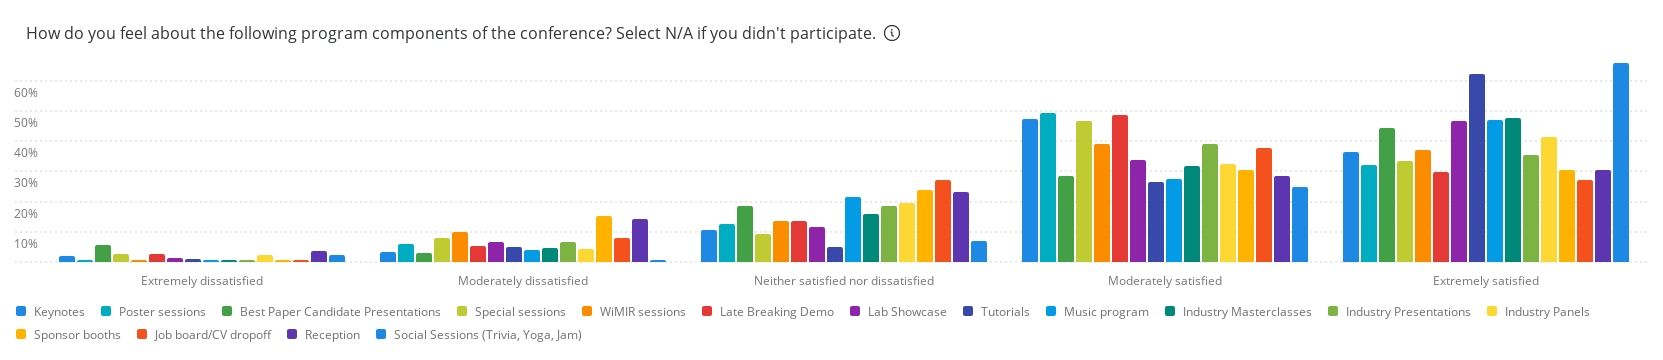
\includegraphics[width=\columnwidth]{fig/survey_satisfaction_item}%
            \caption{Participant satisfaction for individual program items}%
            \label{fig:survey_satisfaction_item}%
        \end{figure}
        %
        The general satisfaction is also indicated by the fact that 69\% of respondents stated that they definitely plan to attend future ISMIR and an additional 24\% state that they will likely attend future ISMIR conferences.
        
        Comparing a virtual conference with a traditional on-site conference shows that a majority of participants feel that the conference participation is more constrained by obligations (mostly work and time zones) as shown in Fig.~\ref{fig:survey_constraints}.
         \begin{figure}%
            \includegraphics[width=\columnwidth]{fig/survey_constraints}%
            \caption{Participant constraints during the conference}%
            \label{fig:survey_constraints}%
        \end{figure}
        
        Figure~\ref{fig:survey_onsite} compares the virutal conference experience with an on-site conference and shows that many of the program items are rated equally or worse for the online-only conference.
          \begin{figure}%
            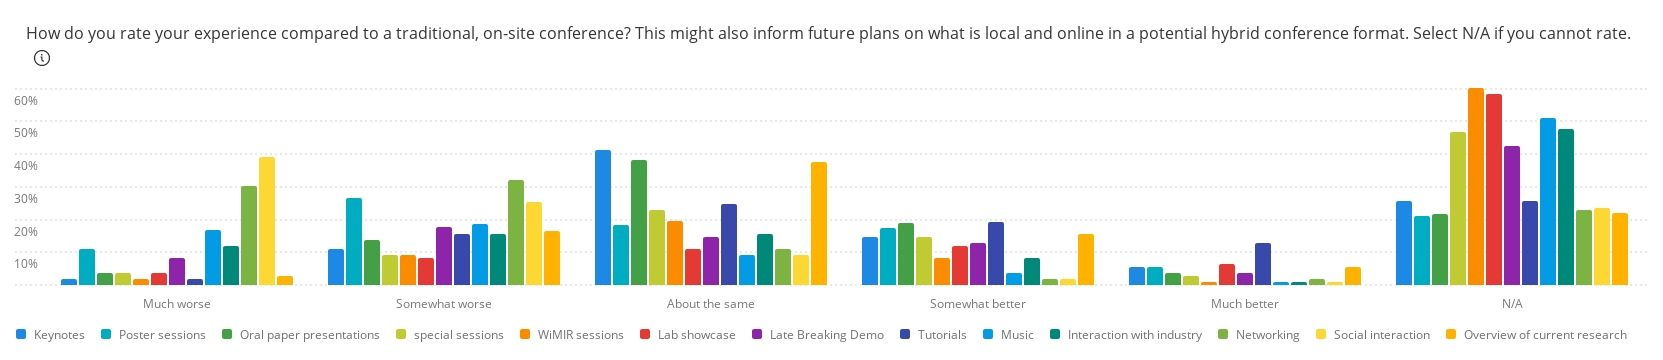
\includegraphics[width=\columnwidth]{fig/survey_onsite}%
            \caption{Virtual conference vs.\ On-site}%
            \label{fig:survey_onsite}%
        \end{figure}

    \subsection{Outlook}
        Survey responses shown in Fig.~\ref{fig:survey_future} indicate that a majority of attendees appreciate the mix of program items and want to keep most items similarly represented in future ISMIR conferences, potentially a bit more of everything. The items that a slightly larger group of attendees wants to emphasize more are Oral Presentations, the social program, as well as D\&I and Newcomer initiatives.
          \begin{figure}%
            \includegraphics[width=\columnwidth]{fig/survey_future}%
            \caption{Emphasis on future program items}%
            \label{fig:survey_future}%
        \end{figure}

    \subsection{Outlook}
        ISMIR had three satellite events (WiMIR workshop, NLP4MusA, and MDX). DLfM, a satellite in previous years, did not communicate any reasons for joining another conference.

        All satellite events were organized largely independent from the main event. While WiMIR did not require any registration, it helped that attendees of the other satellite events registered through the same system similarly to normal ISMIR attendees. In retrospect, the satellite event fees for non-ISMIR participants (registration was free in combination with an ISMIR registration) would not have been necessary; however, at the time of planning there were concerns that the number of satellite participants could potentially be higher than the number of ISMIR participants, so it was decided to charge the platform cost for non-ISMIR attendees.

      


\end{document}
